\title{Changes on CRAN}
\subtitle{2022-04-01 to 2022-06-30}
\author{by Kurt Hornik, Uwe Ligges and Achim Zeileis}
\maketitle

\sloppy

\inputencoding{utf8}

In the past 3 months, 485 new packages were added to the CRAN package
repository.  76~packages were unarchived, 1179 were archived and 3 had
to be removed.  The following shows the growth of the number of active
packages in the CRAN package repository:

\begin{figure}[h]
  \centering
  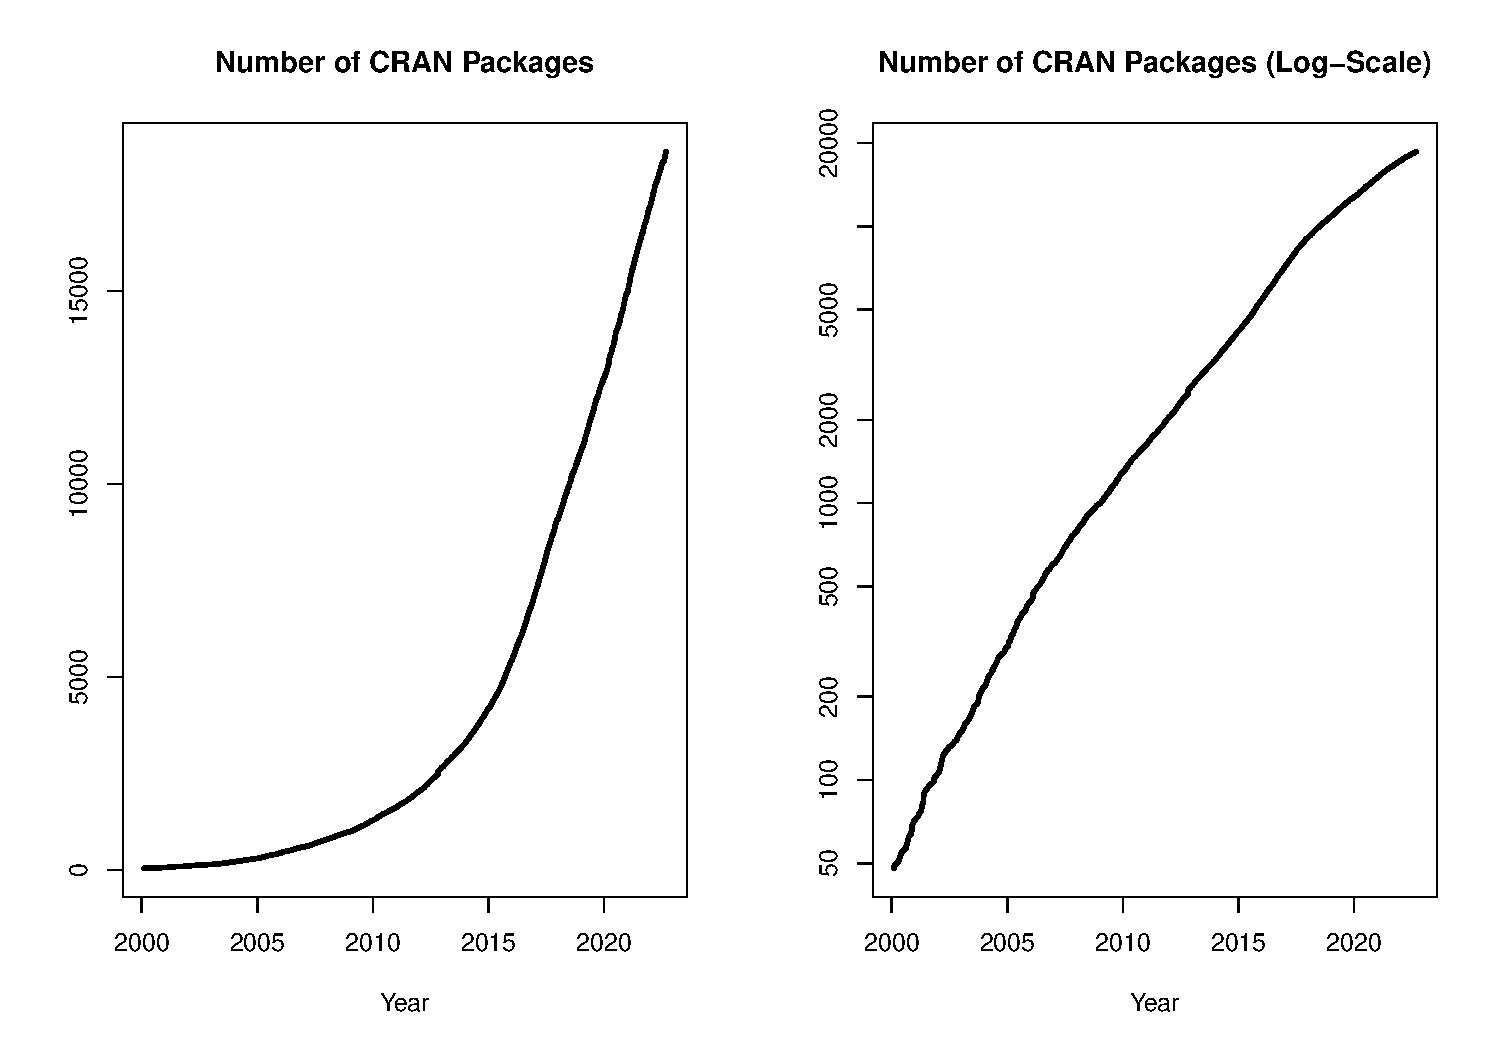
\includegraphics[width=5in]{cran_growth}
\end{figure}

\noindent
On 2022-03-31, the number of active packages was around 18260.

\subsection{Changes in the CRAN Repository Policy}

%% cd ~/src/org/R-project/R-dev-web/CRAN/Policy
%% svn diff -r{2022-04-01}:{2022-08-31}

The
\href{https://CRAN.R-project.org/web/packages/policies.html}{Policy}
now says the following:
\begin{itemize}
 \item The ownership of copyright and intellectual property rights of
  all components of the package must be clear and unambiguous [\ldots]
  ('All components' includes any downloaded at installation or during
  use.)
 \item The package’s \file{DESCRIPTION} file must show both the name and
  email address of a single designated maintainer (a person, not a
  mailing list).  That contact address must be kept up to date, and be
  usable for information mailed by the CRAN team without any form of
  filtering, confirmation \ldots. Forwarding mail from the maintainer
  address increasingly results in confusing non-delivery notifications
  to the original sender, so is best avoided.
 \item Security provisions must not be circumvented, for example by not
  verifying SSL/TLS certificates.
\end{itemize}

\href{https://CRAN.R-project.org/web/packages/external_libs.html}{External
  Libraries for CRAN packages} now says
\begin{itemize}
 \item For macOS: JAGS may or may not be available.  There is an
  `official' release for both architectures at
  \url{https://sourceforge.net/projects/mcmc-jags/files/JAGS/4.x/}.
 \item For Windows: The build system for Windows changed with 4.2.0 and
  only that is considered here (and only 64-bit Windows is now
  supported).  
\end{itemize}

\subsection{CRAN package submissions}

In the second third of 2022 (May 2022 to August 2022), CRAN received 
9860 package submissions.
For these,  17476~actions took place of which 11354 (65\%) were auto
processed actions and 6122 (35\%) manual actions.

Minus some special cases, a summary of the auto-processed and manually
triggered actions follows:
\begin{center}
  \setlength{\tabcolsep}{2pt}
\begin{tabular}{l|rrrrrrrr}
           &archive& inspect& newbies& pending& pretest& publish& 
recheck& waiting\\ \hline
   auto    &  2559 &   2660 &   1635 &      0 &      0 &   2830 &    933 
&    737\\
   manual  &  2178 &    113 &    568 &    255 &     55 &   2226 &    595 
&    132
\end{tabular}
\end{center}

These include the final decisions for the submissions which were
\begin{center}
\begin{tabular}{l|rr}
action & archive        & publish\\ \hline
auto   &  2462 (25.5\%) & 2311 (23.9\%)\\
manual &  2156 (22.3\%) & 2735 (28.3\%)
\end{tabular}
\end{center}
where we only count those as \emph{auto} processed whose publication or
rejection happened automatically in all steps.

A new team member, Benjamin Altmann, joined the CRAN submission team. 
Welcome, Beni.
Unfortunately, Gregor Seyer left the CRAN submission team after 
processing 5482~incoming submissions. Thanks a lot!

\subsection{CRAN mirror security}

%% ~/Work/R/CRAN_Admin/cran_secure_http_and_rsync.R

Currently, there are 102 official CRAN mirrors, 80 of which provide both
secure downloads via \samp{https} \emph{and} use secure mirroring from
the CRAN master (via rsync through ssh tunnels).  Since the~R 3.4.0
release, \code{chooseCRANmirror()} offers these mirrors in preference to
the others which are not fully secured (yet).

\subsection{CRAN Task View Initiative}

There are three new task views:
\begin{description}
 \item[\href{https://CRAN.R-project.org/view=CausalInference}{CausalInference}]
  Maintained by Imke Mayer, Pan Zhao, Noah Greifer,
  Nick Huntington-Klein, and Julie Josse.
 \item[\href{https://CRAN.R-project.org/view=Epidemiology}{Epidemiology}]
  Maintained by Thibaut Jombart, Matthieu Rolland, and Hugo Gruson.
 \item[\href{https://CRAN.R-project.org/view=SportsAnalytics}{SportsAnalytics}]
  Maintained by Benjamin S. Baumer, Quang Nguyen, and Gregory J. Matthews.
\end{description}

Currently there are 39 task views (see
\url{https://cran.r-project.org/web/views/}), with median and mean
numbers of CRAN packages covered 101 and 112, respectively.  Overall,
these task views cover 3668~CRAN packages, which is about 20\% of all
active CRAN packages.

\address{Kurt Hornik \\
  WU Wirtschaftsuniversit\"at Wien, Austria \\
  \email{Kurt.Hornik@R-project.org}}

\address{Uwe Ligges \\
  TU Dortmund, Germany \\
  \email{Uwe.Ligges@R-project.org}}

\address{Achim Zeileis \\
  Universit\"at Innsbruck, Austria \\
  \email{Achim.Zeileis@R-project.org}}

